\newpage
\section{Introduction}
\label{ch:Introduction}

% \paragraph*{Literature for this section:} \begin{itemize}
%     \item "An Introduction to Self-adaptive Systems: A Contemporary Software Engineering Perspective" \cite{SasIntroduction}
%     \item "Software Engineering for Self-Adaptive Systems: A Research Roadmap" \cite{ResearchRoadmap}
%     \item "Software Engineering for Self-Adaptive Systems: A Second Research Roadmap" \cite{SecondResearchRoadmap}
%     \item "Claims and supporting evidence for self-adaptive systems: A literature study" \cite{ClaimsAndSupportingEvidence}
%     \item "Self-Adaptive Software: Landscape and Research Challenges" \cite{LandscapeAndResearchChallenges}
% \end{itemize}

\begin{figure*}[hbt!]
    \centering
    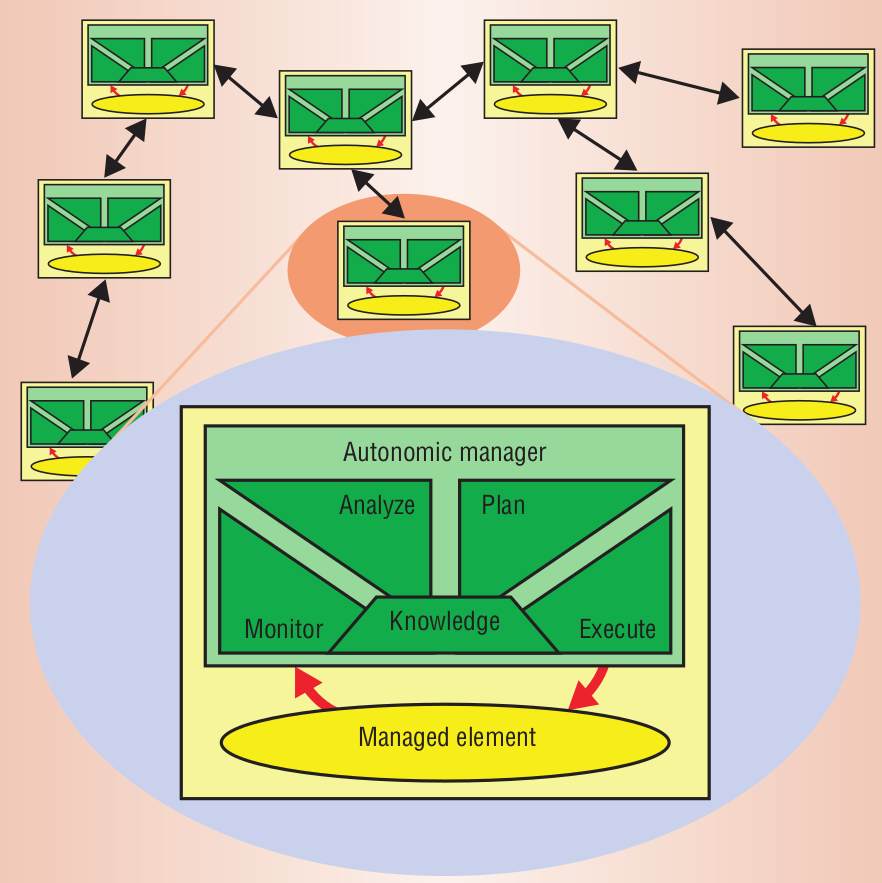
\includegraphics[width=0.6\textwidth]{images/MAPEK.png}
    \caption{The MAPE-K (Monitor-Analyze-Plan-Execute with Knowledge) feedback loop by Kephart and Chess, 2003 \cite*{VisionOfAutonomicComputing}}
    \label{fig:MAPEK}
\end{figure*}

% TODO: What are Self-Adaptive Systems?}
% TODO: Why are Self-Adaptive Systems useful?}
The complexity of modern software systems is constantly growing.
Most of this growth in complexity stems from the
"need to integrate several heterogeneous environments into corporate-wide computing systems, 
and to extend that beyond company boundaries into the Internet" (Kephart and Chess, 2003 \cite*{VisionOfAutonomicComputing}).
This has reached a state where the 
"complexity appears to be approaching the limits of human capability" (Kephart and Chess, 2003 \cite*{VisionOfAutonomicComputing}).
In combination with the uncertainty about a software systems future operations and environment,
that the developers of such complex systems face, it becomes uneconomical to purely operate such a system by human operators.
\newline
\par


From this the need for software systems which can autonomously manage themselves arises.
In order to achieve this task of autonomous self-management, the system has to be able to:
% MAPE-K -> Monitor, Analyze, Plan, Execute with Knowledge
\begin{itemize}
    \item detect faults and changes in its environment.
    \item decide how to react to faults and changes in the systems environment.
    \item make changes to itself.
\end{itemize}

To model these abilities Kephart and Chess developed
the MAPE-K (Monitor-Analyze-Plan-Execute with Knowledge) feedback loop \cite*{VisionOfAutonomicComputing} in Figure \ref{fig:MAPEK}.
\paragraph*{Monitor} First the system has to monitor itself and its environment. 
\paragraph*{Analyze} The data, gathered by the monitoring step, has to be analyzed to detect changes and faults.
\paragraph*{Plan} If the analyzing step detects, that an adaptation is necessary, 
the planning step plans which changes have to be made.
\paragraph*{Execute} After the changes have been planned, they need to be executed.
\paragraph*{Knowledge} All of this happens with Knowledge of the environment and the system.
\newline
\par


Software systems that can autonomously manage themselves are called Self-Adaptive Systems
because of their ability to adapt themselves.
\newline
\par


% This approach to managing software systems has advantages compared to the use of human operators:
% \begin{itemize}% TODO: list advantages.
%     \item 
% \end{itemize}

% TODO: What are the limits of Self-Adaptive Systems?}
% TODO: The need for optimizing Self-Adaptive Systems}
While Self-Adaptive Systems are better at handling more complex systems,
human operators are better at handling uncertainty.
Because the rules and policies, used by Self-Adaptive Systems,
are statically created at the design time of the system, a Self-Adaptive System can adapt its underlying system to a changing environment,
but it can not adapt its own adaptation process.
This leads to an increasing divergence between the expected results of adaptations and the actual results,
when the environment changes in ways that were not predicted by developers during the design time of the system.
\newline
\par


From this the need for optimizations for Self-Adaptive Systems arises.
While there already are many Optimization Approaches for Self-Adaptive Systems,
there is no classification for these Optimization Approaches.
Because of this, the existing Optimization Approaches can not be easily compared
and it is difficult to identify areas that require further research.
This paper aims to provide such a classification for Optimization Approaches for Self-Adaptive Systems
\newline
\par


To derive a classification for Optimization Approaches for Self-Adaptive Systems,
the second chapter will first explain how Self-Adaptive Systems are classified
using three different approaches.
Based on these approaches, a classification for Optimization Approaches for Self-Adaptive Systems will be derived
and explained in the third chapter.
The fourth chapter applies the classification to some existing Optimization Approaches
and compares them using the classification.
